\subsection{Organização do projeto}
Assim como o backend o modelo a seguir para o frontend foi o MVC. 

Como recomendado de boas práticas de código limpo da framework as cores do tema da aplicação foram todas colocadas em um ficheiro separado de forma a garantir que a troca de tema da aplicação é facilitada. Outras aplicações de boas práticas de código limpo foram, sempre que possível particionar o código das páginas em vários widgets de forma a ser de fácil navegação e também a criação de widgets reutilizaveis de forma a evitar a repetição de código e também para agilizar o desenvolvimento de código. Sendo assim a estrutura do projeto foi organizada da seguinte forma:
\begin{figure}[htb]
  \centering
  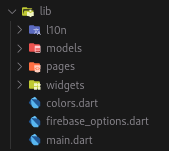
\includegraphics[width=0.35\textwidth]{images/implementacao/frontend/organizacao_projeto.png}
  \caption{Organização do projeto}
  \label{fig:69}
\end{figure}

\begin{itemize}
  \item \textbf{l10n} - Traduções da aplicação;
  \item \textbf{models} - Modelos de classes como handlers, helpers, providers, entre outros;
  \item \textbf{pages} - Páginas da aplicação;
  \item \textbf{widgets} - Widgets referentes às páginas;
\end{itemize}
\vspace{60mm}

